%\documentclass{article}
%\usepackage[utf8]{inputenc}

\documentclass[12pt]{article}
\usepackage{graphicx} % This lets you include figures
\usepackage{hyperref} % This lets you make links to web locations
\graphicspath{ {./images/} }

\usepackage[rightcaption]{sidecap}
\usepackage{subcaption}
\usepackage{wrapfig}
\usepackage{amsmath}
\usepackage{float}

\usepackage{enumitem}

\usepackage{lipsum}

\usepackage{imakeidx}

\makeindex

\title{Data Driven Kinetics - Manual}
\author{Pragneshkumar Rana, Sivaram Ambikasaran, Krithika Narayanaswamy}
\date{\today}

\begin{document}
\maketitle{}

\tableofcontents
\listoffigures
\clearpage
\newpage

\section{Introduction:}


\subsection{Ignition delay brief intro:}


 Chemical reaction and transport process are main components of the combustion process. In combustion, chemical reaction have different time scales which is called as a ignition delay. It is also major combustion property. Ignition delay can be divided into two parts: 
 \begin{enumerate}
 	\item Physical Ignition Delay 
 	\subitem Physical ignition delay depends on different physical phenomenon of combustion process such as, atomization of fuel, heating, evaporation rate of fuel, etc.
 	\item Chemical Ignition Delay
 	\subitem Chemical ignition delay depends on type of fuel, molecular structure of fuel, equivalence ratio etc. 
 \end{enumerate} 
 
 \subsection{Why ignition delay?} 
 Ignition delay is crucial parameter for combustor and IC engines. Right amount of ignition delay is essential for efficient working of such devices. Calculation of ignition delay is computationally intensive as it requires time consuming simulations which includes detailed complex chemistry as well. To resolve such issue; accurate, simplified, and efficient framework has been designed to predict the ignition delay. To predict ignition delay, shock tube data of n-alkanes is utilized. 

\subsection{Key-idea behind framework:} \label{sec:key_idea}
The goal of a framework is to predict ignition delay. For that, machine learning concepts, multiple linear regression is used along with concept of the recursive tree. To divide the data based on error, tertiary tree is utilized. The whole process is summarized briefly below:

 \begin{enumerate}
	\item Fit regression plane on all the fuel data using multiple regression.
	\item Calculate relative error of the actual and predicted value for all data.
	\item Data points which has relative error less than specified criteria will be combined in one bin called \textbf{center cluster}
	
	\item Other data, which has relative error more than  specified criteria will be further bifurcated based on absolute error of actual and predicted value.
	
	\item Data points which has positive absolute error has lies on one side of the fitted plane and other data points which has negative sign lies on other side of the fitted plane.
	
	\item Thus, three clusters will be obtained in which,
	\subitem \textbf{Left cluster} : Data points which has relative error more than specified error and actual error has positive sign.
	
	\subitem \textbf{Center Cluster} : Data points which has relative error less than specified criteria.
	
	\subitem \textbf{Right Cluster} : Data points which has relative error more than specified error and actual error has negative sign. 
 \end{enumerate} 
 	Center cluster will give a correlation for the data and will not be divided further. Whereas, Left and Right cluster may also give correlation if they satisfies the specified relative error criteria, otherwise it will be divided recursively by following step:1-6 until specified relative error criteria is not fulfilled. 
 	
 \begin{figure}[H]
     \centering
     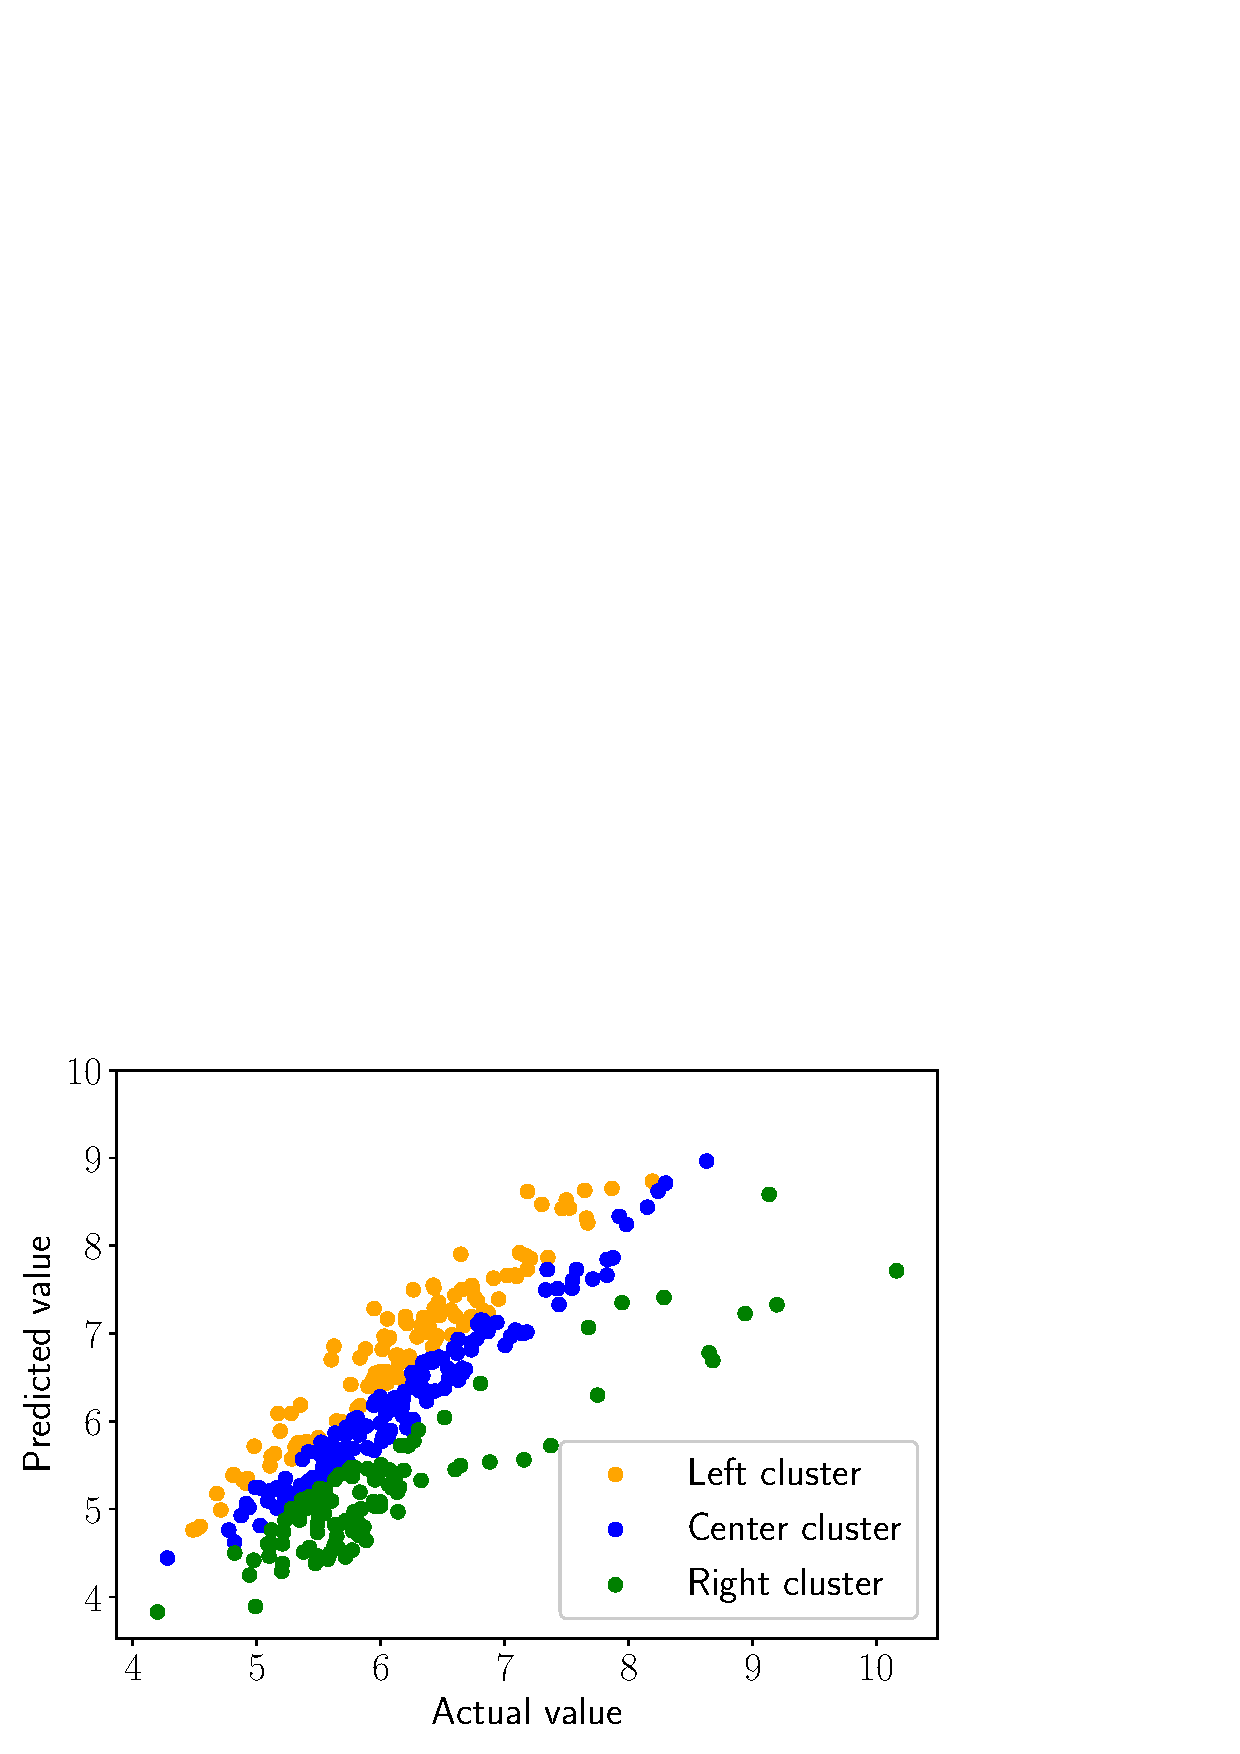
\includegraphics[width=0.63\textwidth]{images/cluster_visulization_0.png}
     \caption{Division of cluster based on Relative Error}
     \label{fig:cluster0}
 \end{figure}

%\clearpage
For example, after fitting the first regression plane, result of the actual and predicted value is shown in fig~\ref{fig:cluster0}. Blue colour shows, the data points which has relative error less than 5\%. Green and orange colored data points have relative error more than 5\%. Apart from relative error, absolute error also plays essential role in clustering. Orange data point have positive absolute error and green data points have negative absolute error. By this way, three clusters is  obtained. Further, orange and green data points will be divided into three clusters individually following the same procedure explained above. Obtained result is shown in fig~\ref{fig:cluster1} and \ref{fig:cluster2}. 
	
\begin{figure}[H]
	\centering
	\begin{subfigure}{.5\textwidth}
		\centering
		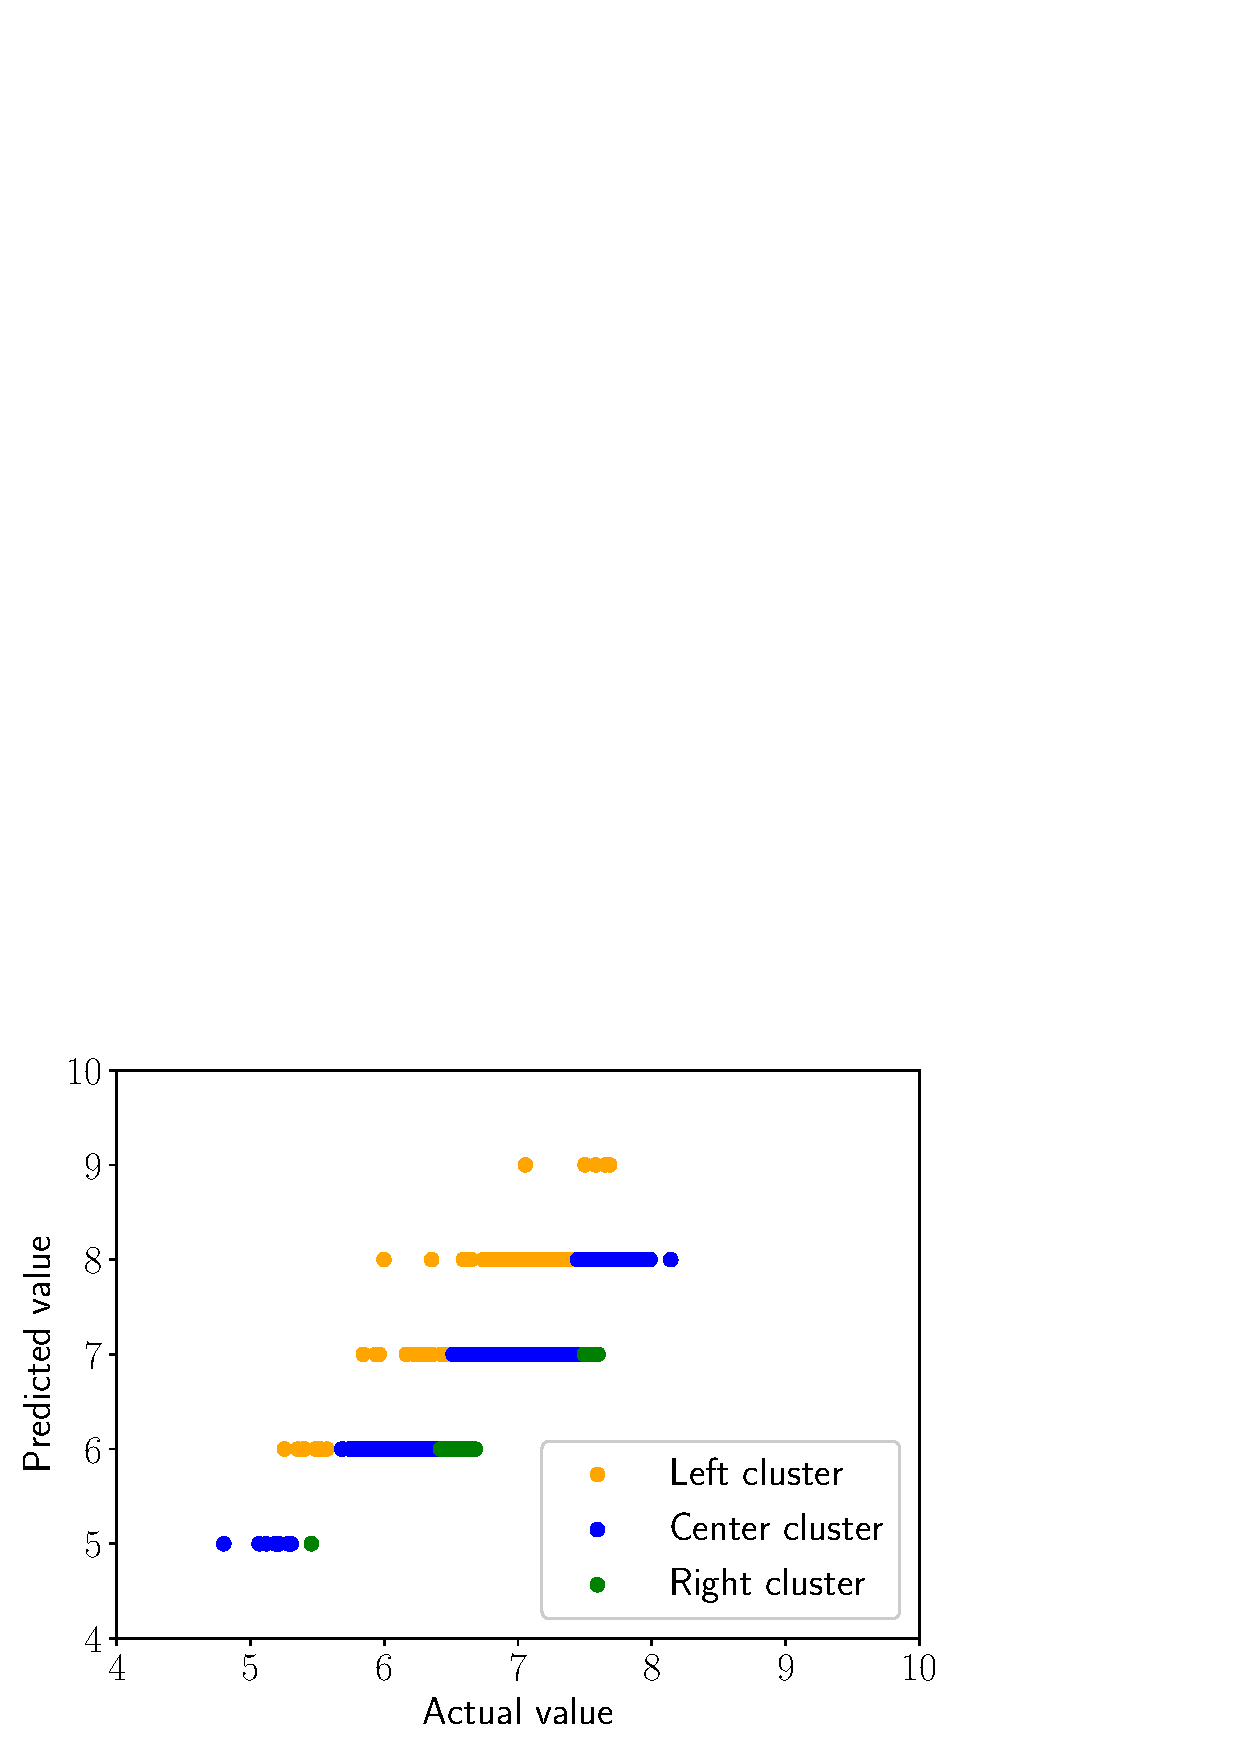
\includegraphics[width=1.1\linewidth]{cluster_visulization_1.png}
		\caption{Left Cluster Division}
		\label{fig:cluster1}
	\end{subfigure}%
	\begin{subfigure}{.5\textwidth}
		\centering
		\includegraphics[width=1.1\linewidth]{cluster_visulization_2.png}
		\caption{Right Cluster Division}
		\label{fig:cluster2}
	\end{subfigure}
	\caption{Division of left and right cluster into sub-clusters}
	\label{fig:test}
\end{figure}

\begin{figure}[H]
 	\centering
 	%left trim
	\includegraphics[trim={2cm 12cm 0 11cm},clip,scale=0.73]{tree.pdf}
 	\caption{Conceptual tree diagram of procedure}
 	\label{fig:tree}
\end{figure}

\textbf{Each center clusters gives one correlation  for prediction of ignition delay.} \textbf{Left and right clusters can also give correlation or can generate cluster if it satisfies the specified relative error criteria} \textbf{else, it will further divide into more parts/clusters till relative error criteria is not satisfied for data-points which is given in fig-\ref{fig:tree}.} For example distribution of data points in different cluster is shown in fig~\ref{fig:datapoints_tree}.

\begin{figure}[H]
	\centering
	%left trim
	\includegraphics[trim={2cm 12.5cm 0 10cm},clip,scale=0.73]{Datasize.pdf}
	\caption{Division of data points in different clusters}
	\label{fig:datapoints_tree}
\end{figure}

Along with that, the regression coefficient obtained  after following the whole procedure is given in fig~.\ref{fig:coef_tree}. From figure~\ref{fig:coef_tree}, it is clear that the nodes highlighted with red borders shows final clusters. The correlation obtained by highlighted clusters as in fig-\ref{fig:coef_tree} are useful for prediction of ignition delay value. Calculation of centroid and distance of data points from those centroid plays major role in prediction. 

The formulation of multiple linear regression used to find out the correlation is given as,
\begin{align}
	\tau &= \beta_0 \frac{P}{P_0}^{\beta_1} X_{fuel}^{\beta_2} X_{oxi}^{\beta_3} exp \bigg({\beta_4 \frac{T_0}{T} + \beta_5 \frac{T_0}{T \times C_{SH}}}\bigg) \\
	 &= \beta_0 \frac{P}{P_0}^{\beta_1} X_{fuel}^{\beta_2} X_{oxi}^{\beta_3} exp \bigg(\frac{1}{T}\bigg\{\underbrace{\beta_4 {T_0} + \beta_5 \frac{T_0}{C_{SH}}}_\text{similar to $\frac{E_a}{R}$}\bigg\}\bigg)
\end{align}		 

Here, all the $\beta_i$ values indicates the regression coefficients. {P-pressure, $X_{fuel}$-fuel mole fraction,$ X_{oxi}$-oxidizer mole fraction, T-temperature, $C_{SH}$-number of secondary carbon and hydrogen bonds} are the features of the equation. $P_0$ and $T_0$ are reference pressure and temperature. 

\begin{figure}[H]
	\centering
	%left trim
	\includegraphics[trim={2cm 7cm 0 3cm},clip,scale=0.9]{coefficient.pdf}
	\caption{Coefficient obtained in different clusters after regression. Highlighted nodes of tree indicates final clusters which are useful of prediction.}
	\label{fig:coef_tree}
\end{figure}

\section{Setting up for the first time:} \label{sec:setup}
{
	\begin{itemize}
		\item After downloading the application, put it in the $./home$ directory. 
		\item Install all the dependency. Dependency can be directly installed using INSTALL.sh file. They are mentioned below: 
		\begin{itemize}
		\item numpy
		\item matplotlib
		\item seaborn
		\item \href{https://scikit-learn.org/stable/install.html}{scikit}
		\item \href{https://www.statsmodels.org/stable/install.html}{statmodel}
		\item \href{https://www.rdkit.org/docs/Install.html}{rdkit}
		\item \href{https://gist.github.com/rain1024/98dd5e2c6c8c28f9ea9d}{latexpdf} - Install manually by following instruction

	\vspace{0.5cm}
	
		To install all dependency run the following command:
		\item chmod +x INSTALL.sh
		\item ./INSTALL.sh
		
		\end{itemize}
		
		\item After installing all the dependency, open .bashrc file and copy-paste following command at end of the file.
		
		\begin{itemize}
			\item $\#\#$For DATA DRIVEN FRAMEWORK
			\item export IDCODE="\text{$\sim$/Data\_driven\_Kinetic}/"
			\item export PATH=\$PATH:\$IDCODE
			\item alias IDprediction="\text{pwd$\>\sim$/Data\_driven\_Kinetics/filelocation.txt  \&\&  Run.sh}"
		\end{itemize}
	\item All set! - Run the application following instruction given in section-\ref{sec:run}
	\end{itemize}
		
}

\newpage

\section{Run the App:} \label{sec:run}
	After following the procedure given in section-\ref{sec:setup}, it is convenient to use the app from any directory. let's consider filename- \textbf{alkane.csv} for explanation of all commands.  
	\begin{itemize}
		\item Command to run the code:
		\subsubitem \textbf{IDprediction -flag File-Name }
	\end{itemize}
	\subsection{Available options and flags:}
	\vspace{0.4cm}
	\noindent
	
	\begin{itemize}[wide = 0pt, labelwidth = 1.3333em, labelsep = 0.3333em, leftmargin = \dimexpr\labelwidth + \labelsep\relax ]%
	\item \textbf{-a : \textit{Analyze} the data-set by selecting range of parameters}\\
	
	\begin{itemize}[wide = 0pt, labelwidth = 1.3333em, labelsep = 0.3333em, leftmargin = \dimexpr\labelwidth + \labelsep\relax ]%
	\item command : \textbf{IDprediction -a alkane.csv} \\
	\item To analyze and find out data-points having properties in certain range to analyze ignition delay for specific fuel.
	\begin{itemize}
		\item select fuel by giving corresponding index as input 
		\item Input equivalence-ratio  from available options
		\item Input pressure value from available options
		\item By default it will considers all the data points having same fuel structure and same equivalence ration within $\pm$0.5 atm. If you want to change the range pressure input:'y' and input the desired range else input:'n' \\
	\end{itemize}
	
	\item \textbf{Output :}
	\begin{itemize}
		\item  ./result/data$\_$analysis/
		\subitem  It will generate the plot of $\tau$ vs 1000/T, which includes data points having selected $\phi$, specified range of pressure for selected fuel.
	\end{itemize}
	\end{itemize}


		\newpage
			\item \textbf{-b : \textit{Bond} types in given fuel} \\
			\begin{itemize}
				\item command : \textbf{IDprediction -b CCCC} 
				\subitem To find out type of chemical bonds available in different type of carbon and other atoms. \\
			\textbf{Note: Works for n-alkanes and branched alkanes.}
				\item \textbf{Output :}
				\begin{itemize}
						\item ./result/Bond\_details/
						\subitem It will generate \textbf{SMILE\_result.csv} file which contains available
						bond details for given fuel. Detail in the file includes, 
						\begin{itemize}
							\item  \textbf{Primary\_C} : Total number of primary carbons 
							\item  \textbf{Secondary\_C} : Total number of secondary carbons 
							\item  \textbf{Tertiary\_C} : Total number of tertiary carbons 
							\item  \textbf{Quaternary\_C} : Total number of Quaternary carbons 
							\item  \textbf{Other\_Atom} : Total number of atoms other than carbon 
							\item  \textbf{P\_P} : Total number Primary-Primary carbon bonds 
							\item  \textbf{P\_S} : Total number Primary-Secondary carbon bonds 
							\item  \textbf{P\_T} : Total number Primary-Tertiary carbon bonds 
							\item  \textbf{P\_Q} : Total number Primary-Quaternary carbon bonds 
							\item  \textbf{S\_S} : Total number Secondary-Secondary carbon bonds 
							\item  \textbf{S\_T} : Total number Secondary-Tertiary carbon bonds  
							\item  \textbf{S\_Q} : Total number Secondary-Quaternary carbon bonds 
							\item  \textbf{T\_T} : Total number Tertiary-Tertiary carbon bonds 
							\item  \textbf{T\_Q} : Total number Tertiary-Quaternary carbon bonds 
							\item  \textbf{Q\_Q} : Total number Quaternary-Quaternary carbon bonds 
							\item  \textbf{P\_H} : Total number Primary carbon - Hydrogen bonds 
							\item  \textbf{S\_H} : Total number Secondary carbon - Hydrogen bonds 
							\item  \textbf{T\_H} : Total number Tertiary carbon - Hydrogen bonds 
							\item  \textbf{Fuel} : Fuel SMILE \\
						
						\end{itemize}
					\textbf{		\textbf{Note} : If file already exits then result will be appended to old output file.}
				\end{itemize}
				
				
			\end{itemize}
			
		
		\newpage
		
			\item \textbf{-h : \textit{Histogram} plots of parameters for each fuel individually } \\
			\begin{itemize}
			\item command : \textbf{IDprediction -h alkane.csv} 
			\subitem   It will generate the histogram plots of parameters associated with ignition delay, separately for all the fuels. \\
			\item \textbf{Output :}			
			\begin{itemize}

					\item   ./result/Fuel\_Parameter\_Histogram/
					\subitem	Directory contains, folders named by fuel smiles. Each folder contains histogram plot of parameters associated with ignition delay. These plots are useful for visualization and analysis of the parameters. 	
			\end{itemize}
				\end{itemize}
			


			
		\item \textbf{-c : \textit{Criteria} for separation } \\
		
			\begin{itemize}

				\item command : \textbf{IDprediction -c 0.05 -m alkane.csv} 
				\subitem Flag has to be passed with multiple  linear regression or error based clustering regression. Criteria value 0.05 indicates relative error of 5\%. Criteria plays key role in creation of clusters. Use of criteria is to filter out the data points which has relative error less than specified value to create a cluster.	
				\item \textbf{Default : 0.05	}		
			\end{itemize}
			
		\item \textbf{-r : \textit{Remove} feature by back-elimination } \\
				\begin{itemize}

					\item command : \textbf{IDprediction -c 0.05 -r True -s 0.05 -m alkane.csv} \\
					\subitem This Flag \textbf{has to be passed with True or False  }.
				\subsubitem	True : Backward elimination will be activated 
				\subsubitem	Flase : Backward elimination will be deactivated \\
				\item \textbf{	Default : False }\\
				
				\end{itemize}
				
			\newpage
			
		\item \textbf{-s : \textit{Significance Level} for p-value or Confidence zone criteria } \\
		
			\begin{itemize}
				\item command : \textbf{IDprediction -c 0.05 -r True -s 0.05 -m alkane.csv} 
				\subitem Value passed with this flag is useful for backward elimination. Significance level is used for rejection/acceptance of null hypothesis. Low significance value is generally passed as it indicates higher evidence is needed for rejection of null hypothesis. 
				\item \textbf{Default : 0.05}				
			\end{itemize}
		
		\item \textbf{Null hypothesis :} For multiple linear regression, null hypothesis defined as, there is no statistical relationship between independent and dependent variables or coefficient associated with dependent variable is zero.	\\
		
		
		\item  	\textbf{Backward elimination :} In this procedure, if any feature has p-value more than specified or default value 0.05 (if -r True and -s not passed) then that feature will be eliminated. Result will be obtained running regression again. Same procedure will  be repeated till p-value associated with all the regressor are less then specified value.\\
	
		\item \textbf{-m : \textit{Multiple} linear regression of data } \\
		
			\begin{itemize}		
				\item command : \textbf{IDprediction -c 0.05 -r False -m alkane.csv} 
 \subsubitem \hspace{0.5cm} or \textbf{IDprediction -m alkane.csv} 
				\subitem It will do multiple regression on whole data-set and  will \textbf{generate output as root of the tree.} Details of other flag is mentioned above. If others flags are not passed then it will take default value as mentioned. \\
				
				\item \textbf{Output :}
				\begin{itemize}
					\item \textit{ ./object\_file/} - useful for prediction  
					\subitem  This directory has three more sub-directory inside it; \textbf{./regressor -} object file of trained model. \textbf{./x\_names} - has feature names of trained model. \textbf{./scalar}- object file which has function to scale data (NOT UTILIZED). 
					
					\item \textit{ ./result/coefficients/Node\_type/}
					\subitem  stores coefficient obtained after multiple regression  \\
					
					\item \textit{-- ./result/console\_output/Node\_type/}
					\subitem  Output printed on console screen also get stored in the \textbf{output\_result.txt} file \\
					
					\item \textit{ ./result/Node\_type/ID\_comparison\_i/}
					\subitem Directory contains \textbf{./ID\_comparison\_i} folder, which contains file named,
					\textbf{ID\_comparison\_test\_i.csv} which has Ignition delay comparison detail for testing and likewise similar detail of training data is in \textbf{ID\_comparison\_train\_i.csv} file. Ignition Delay comparison file contains y\_act(Actual Ignition Delay value), y\_predicted(Predicted Ignition Delay value), and relative error between those two values.\\
					
					\item \textit{ ./result/vif/Node\_type/}
					\subitem VIF(Variation Inflation Factor) - it is useful to  check the multi-collinearity of the features \\
					VIF = 1 means feature has no multi-collinearity  \\
					VIF = 1-5 means feature has moderate correlation  \\
					VIF $>$ 5  means poorly identify the coefficient \\
					\textbf{./vif\_i.csv} contains features and associated VIF values. \\
					
					source: \\
					\href{https://statisticalhorizons.com/multicollinearity}{Multicollinearity}\\  \href{https://www.statsmodels.org/stable/generated/statsmodels.stats.outliers\_influence.variance\_inflation\_factor.html}{VIF} \\
					
					\textbf{Note: i here indicated index\\
						Node Type includes : \{root,left\_node, center\_node, right\_node\}}

				\end{itemize}
			
				
			\end{itemize}
			
			\newpage
			
			\item \textbf{-t : \textit{Tree -} Error based clustering  regression } 
			\begin{itemize}

				\item command : \textbf{IDprediction -c 0.05 -r False -t alkane.csv} 
				\subsubitem \hspace{0.5cm} or \textbf{IDprediction -c 0.05 -t alkane.csv} 
				
				\subitem The whole idea behind error besed clustering is explained in section-\ref{sec:key_idea}. 
				
				\item \textbf{Output :}
				\begin{itemize}
					\item \textit{ ./object\_file/} -useful for prediction 
					\subitem  This directory has Four more sub-directory inside it;
					\begin{itemize}
						\item \textbf{./regressor -} object file of trained model.
						
						\item \textbf{./x\_names} - feature names of trained model. 
						
						\item \textbf{./scalar} - object file which is used to scale the data (NOT UTILIZED) 
						
					  \item 	\textbf{./centroid}- it contains files for final clusters (highlighted nodes as in fig-\ref{fig:coef_tree}). Each file contains average calculated value of features associated with cluster-data. \\
					\end{itemize} 
					
					
					
					\item \textit{ ./plots/} 
					\subitem  Directory contains several tree based plots which helpful for visualization. Along with that it has sub directory named \textbf{ ./cluster\_plot\_y} which includes comparative plots of $y_{actual}$ vs $y_{predicted}$ for every clusters as shown in fig-\ref{fig:cluster0};
					
					 \textbf{./plots/} directory has six plots. All plots are generated with the help of latex. 
					 \begin{itemize}
						 \item \textbf{ChildLabel} plot is shows index associated with clusters. 
						 \item \textbf{Datasize} plot shows number of data points in each cluster. 
						 \item \textbf{Training} plot shows R2 value of training set in each cluster. 
						 \item  \textbf{Testing} plot shows R2 value of testing set in each cluster.  
						 \item \textbf{MaxRelError} plot shows maximum relative error of training set for each cluster. 
						 \item \textbf{coefficient} plot shows coefficient obtained after regression for each cluster node.
					 \end{itemize}
					
					\textbf{./plots/cluster\_plot\_y/}- it contains plots as in fig-\ref{fig:cluster0}. Plots are useful to understand role of relative error and absolute error in clustering. Data points with same colour are in one cluster. \\
					
					\item \textit{ ./result/coefficients/Node\_type/}
					\subitem  stores coefficient obtained after multiple regression  \\
					
					\item \textit{ ./result/cluster\_data\_before\_regression/Node\_type}
					\subitem  Directory contains cluster specific data-file of \textbf{useful clusters -} means data which is utilized for generation of cluster. \\
					
					\item \textit{ ./result/Tree\_coefficient\_result/Node\_type/}
					\subitem  stores coefficient obtained after multiple regression which is same as copy of ./result/coeffcients/. Stored seperatly as it will not mix its result with Multiple regression result. \textbf{It has data of only final clusters.} \\
					
					\item \textit{ ./result/final\_cluster/Node\_type}
					\subitem  contains data file of seperated clusters for all the nodes \\
					
					\item \textit{ ./result/console\_output/Node\_type/}
					\subitem  Output printed on console screen also get stored on the in the output\_result.txt file \\
					
					\item \textit{ ./result/Node\_type/ID\_comparison/}
					\subitem Directory contains ./ID\_comparison\_i folder, which has Ignition delay comparision files training and testing. Ignition delay comparison file contains y\_act(Actual Ignition delay value), y\_predicted(Predicted Ignition Delay value), and relative error .\\
					
					\item \textit{ ./result/vif/Node\_type/}
					\subitem VIF(Variation Inflation Factor) - To  check the multi-collinearity of the features \\
					VIF = 1 means feature has no multi-collinearity  \\
					VIF = 1-5 means feature has moderate correlation  \\
					VIF $>$ 5  means poorly identify the coefficient \\
					./vif\_i.csv contains features and associated VIF values. \\
					source: 				\href{https://statisticalhorizons.com/multicollinearity}{Multicollinearity},  \href{https://www.statsmodels.org/stable/generated/statsmodels.stats.outliers\_influence.variance\_inflation\_factor.html}{VIF} \\
					
					\textbf{Note: i here indicated index\\
						Node Type includes : \{root,left\_node, center\_node, right\_node\}}\\
				\end{itemize}
			
			\end{itemize}

			
			\item \textbf{-e : \textit{External} Dataset used for prediction of ignition delay  } \\
			
			\begin{itemize}

				\item command : \textbf{IDprediction -e testset.csv} \\
				
				\subitem testset.csv file may contain all the features except ignition delay values. The goal of the process is to predict ignition delay.
				Procedure behind code is briefly mentioned below:,
				\begin{enumerate}
					\item Load all the centroid files 
					\item Calculate the distance of all the data points from all the centroids and assign the centroid to each data point by least distance.
					\item By assigned cluster, load the respective regressor object of that cluster and predict the ignition delay and process the result.
				
				\end{enumerate}								
			\item \textbf{Output :}

				\begin{itemize}
					\item \textit{--./external\_test\_result/console\_output/}
					
					Directory contains \textbf{output\_result.txt } which contains output printed on console screen.\\
					
					\item \textit{--./external\_test\_result/Ignition\_delay\_comparison/}
					
					 {ID\_comparison\_external\_cluster\_\{Node\_index\}\_\{Node\_type\}.csv} file which includes y\_predicted - Predicted Ignition delay value, y\_actual - actual ignition delay vales and relative error between them.
					All files are cluster specific means data point in the assigned to one specific cluster.\\
					
					\item \textit{--./external\_test\_result/classified\_data}
					
					Directory contains several data files. Each file is associated with one cluster and it contains independent variable values,class of data points, predicted and actual ignition delay values.\\
					
					\item \textit{--./external\_test\_result/prediction\_comparison\_plots/}
					
					It contains Predicted Ignition Delay vs Actual Ignition Delay plot. Plots are generated using on data points assigned to specific cluster. In short, each plot is related to each cluster.
				\end{itemize}
			
				
			\end{itemize}
			
			\newpage
			
			\item \textbf{-p : \textit{Plot} frequency of the  parameters} \\
		
			\begin{itemize}

				\item command : \textbf{IDprediction -p coefficient.csv} \\
				
				\subitem While running the regression, data points will be splitted randomly. Due to split and change in the data points, obtained coefficient will get affected. To visualize variations in coefficient and find out average coefficient value this command is utilized. Gives result in the form of plot.
				
				Use this command in the directory where coefficient file exist.
			\item \textbf{Output:}
			\begin{itemize}
				\item ./coefficient\_histogram\_plots
				\subitem it contains all histogram plots
				
				\item ./result/
				\subitem  it contains file output\_result.txt which stores output printed on console screen.
			\end{itemize}
			\end{itemize}
			
			
			\end{itemize}

		
\end{document}
